% --- Capítulo IV: Metodología ---
\addcontentsline{toc}{section}{\textbf{CAPÍTULO IV}}
\addcontentsline{toc}{section}{\textbf{METODOLOGÍA}}

\subsection{Tipo y nivel de investigación}

La presente investigación se clasifica por su propósito como Tecnológica Aplicada, dado que busca resolver un problema práctico y concreto: la sobrecarga cognitiva y la desorganización de apuntes en el entorno universitario, mediante el desarrollo de una solución de software (SynapTome). Por su alcance y profundidad, el estudio corresponde a un nivel explicativo-experimental (específicamente, un diseño cuasi-experimental). Este nivel permite no solo describir el ecosistema desarrollado, sino también determinar las relaciones de causa y efecto que la Variable Independiente (el ecosistema basado en RAG, TrOCR y Grafos de Conocimiento) ejerce sobre la Variable Dependiente (la retención de conocimientos, el rendimiento académico y el aprendizaje colaborativo). Como señalan \textcite{Kreijkes2026}, el uso de diseños experimentales en entornos educativos es fundamental para cuantificar de manera objetiva los efectos de las herramientas basadas en LLMs sobre la comprensión lectora y la memoria de los estudiantes.

\subsection{Diseño de la investigación}

Para abordar la complejidad del ecosistema SynapTome, el diseño metodológico se divide en dos vertientes complementarias: un diseño de ingeniería de software y un diseño de validación académica.

\begin{itemize}
  \item Diseño de Ingeniería de Software: Se emplea la metodología ágil Scrum. Según \textcite{Afian2025}, las metodologías ágiles soportan el desarrollo iterativo, la retroalimentación continua y la adaptabilidad, características esenciales para el desarrollo de plataformas de tutoría impulsadas por inteligencia artificial. El desarrollo se estructura en sprints que abarcan la planificación, el diseño, la implementación del backend y los pipelines de IA, y las pruebas continuas de las funciones.
  \item Diseño de Evaluación (Validación): Se utiliza un diseño de tipo pre-test / post-test con un grupo cuasi-experimental. Se mide el desempeño académico (retención de conocimientos) de los estudiantes antes de la adopción del ecosistema SynapTome y, tras un periodo de uso continuo de la herramienta, se aplica un post-test para evaluar el impacto real generado por la plataforma interactiva y colaborativa en la retención del conocimiento y en el fortalecimiento del aprendizaje colaborativo entre pares.
\end{itemize}

\subsection{Descripción ética de la investigación}

El desarrollo y despliegue del ecosistema SynapTome se adhiere a estrictos estándares de ética y privacidad de la información \parencite{Kreijkes2026, Dano2026}. Antes de iniciar las pruebas, se obtiene un consentimiento informado por escrito de los estudiantes de la UNAMBA, garantizando que su participación sea voluntaria y que tengan el derecho de retirarse del estudio en cualquier momento.\\
A nivel técnico, el tratamiento de los datos personales y el contenido de los apuntes manuscritos subidos por los usuarios se gestiona con políticas de seguridad de grado industrial. Para asegurar la protección de los datos en tránsito y en reposo, la arquitectura implementa autenticación segura mediante tokens JWT (JSON Web Tokens) en los endpoints de la API, mientras que toda la información persistente, incluidas las métricas de evaluación y los grafos relacionales, es resguardada en una base de datos PostgreSQL aplicando el encriptado adecuado, evitando el acceso no autorizado y manteniendo la confidencialidad de la información académica y personal \parencite{Upadhyay2026}.

\subsection{Procedimiento}

El procedimiento general de la investigación comprende cinco fases sistemáticas, desde el levantamiento de requisitos hasta la evaluación del sistema "SynapTome" en un entorno real con estudiantes de Ingeniería de Sistemas de la UNAMBA. 

Como parte fundamental de la fase de integración tecnológica, se diseñó e implementó un pipeline de procesamiento asíncrono desacoplado para operativizar la transformación de los apuntes manuscritos analógicos a formato digital de alta fidelidad. Este flujo de trabajo actúa directamente sobre la eficiencia de captura de información y se detalla a continuación:
\begin{enumerate}
    \item \textbf{Preprocesamiento y normalización de imagen}: Se realiza la captura fotográfica del apunte manuscrito por parte del estudiante. La imagen es enviada al servidor donde se aplican filtros de binarización adaptativa de Sauvola, corrección de inclinación (\textit{deskewing}) y reducción de ruido gaussiano para optimizar el contraste de los trazos de tinta.
    \item \textbf{Inferencia autorregresiva (TrOCR)}: La imagen normalizada segmentada en bloques de interés matemático se procesa mediante la arquitectura de aprendizaje profundo TrOCR. El codificador visual de tipo Vision Transformer (ViT) genera los mapas de características latentes que representan los trazos caligráficos. Posteriormente, el decodificador de lenguaje decodifica estos vectores en secuencias de caracteres que representan fórmulas en sintaxis \LaTeX{} válida y texto plano.
    \item \textbf{Sanitización semántica y post-procesamiento}: Se aplica un analizador sintáctico (\textit{parser}) desarrollado para corregir errores comunes de balanceo de llaves, delimitadores matemáticos y etiquetas algebraicas, garantizando que el código de renderizado sea completamente válido y almacenable en PostgreSQL como un nodo estructurado.
\end{enumerate}

Este pipeline de IA se ilustra en la Figura \ref{fig:mi_diagrama_clave}.

\begin{figure}[H]
    \centering
    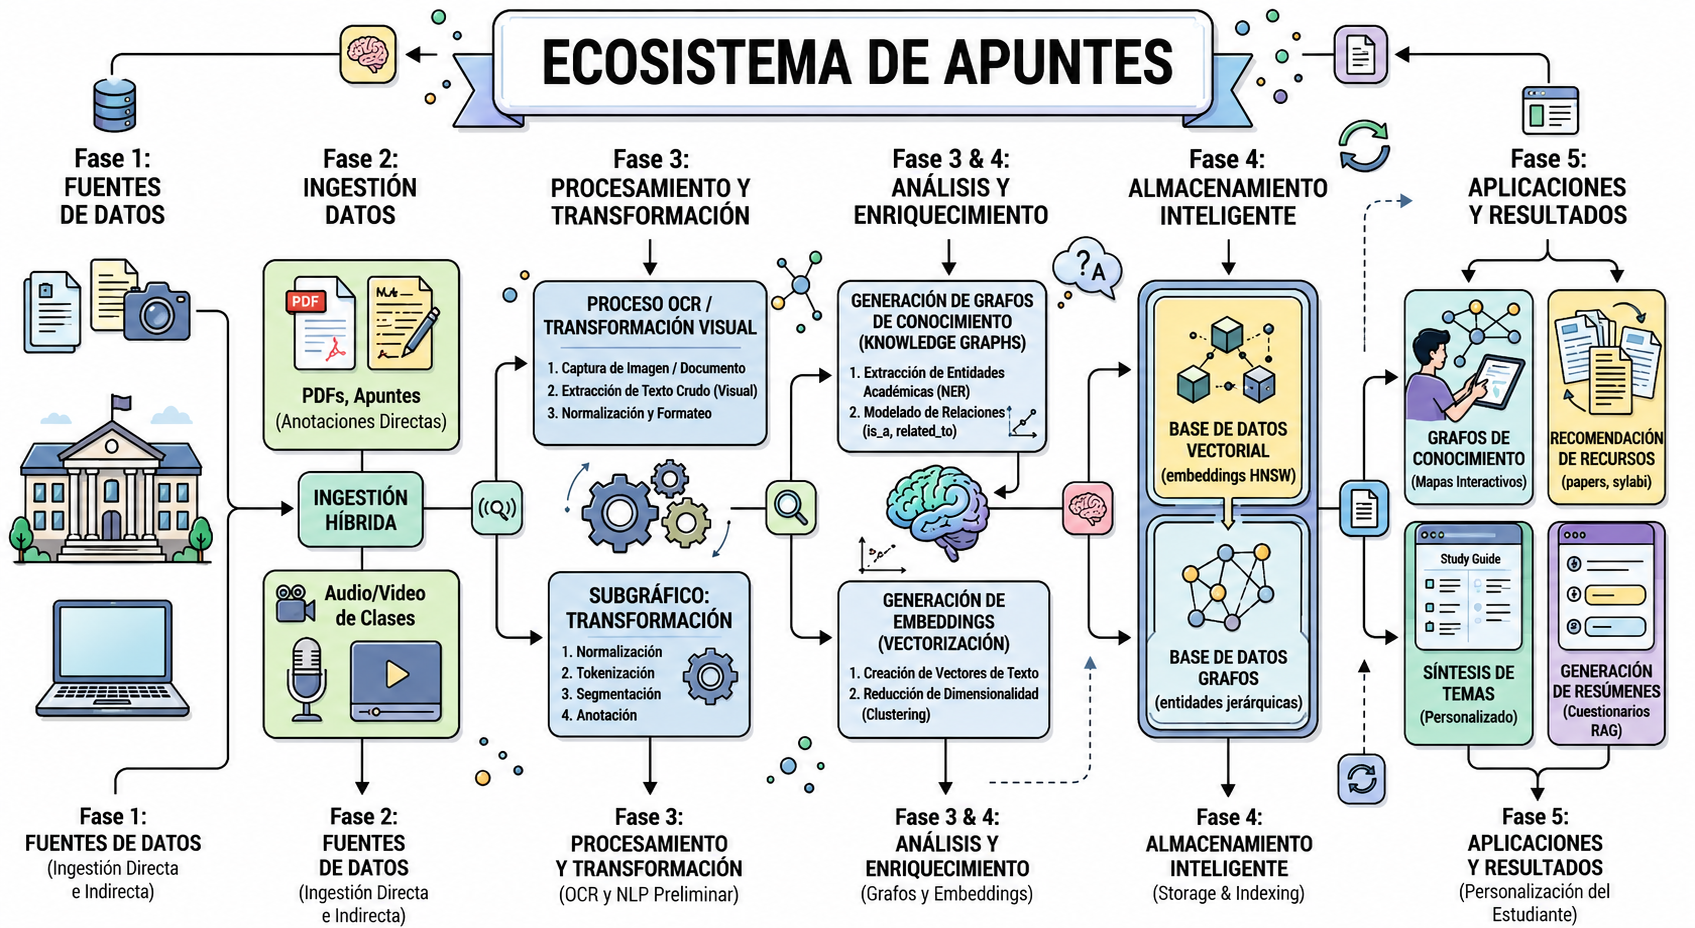
\includegraphics[width=0.85\textwidth]{pipeline.png}
    \caption{Pipeline adaptativo de transcripción caligráfica manuscrita (HTR) e integración RAG/Grafo en el ecosistema SynapTome.}
    \label{fig:mi_diagrama_clave}
\end{figure}

Las actividades específicas, tecnologías empleadas y entregables documentados para cada una de las fases de la investigación se detallan en la Tabla \ref{tab:procedimiento}.

\begin{table}[H]
\centering
\caption{Fases del procedimiento de investigación}
\label{tab:procedimiento}
\scriptsize % Se reduce ligeramente a scriptsize para que el contenedor TikZ con borde grueso no sufra desbordes de margen

\renewcommand{\arraystretch}{1.3}
\setlength{\tabcolsep}{4pt}

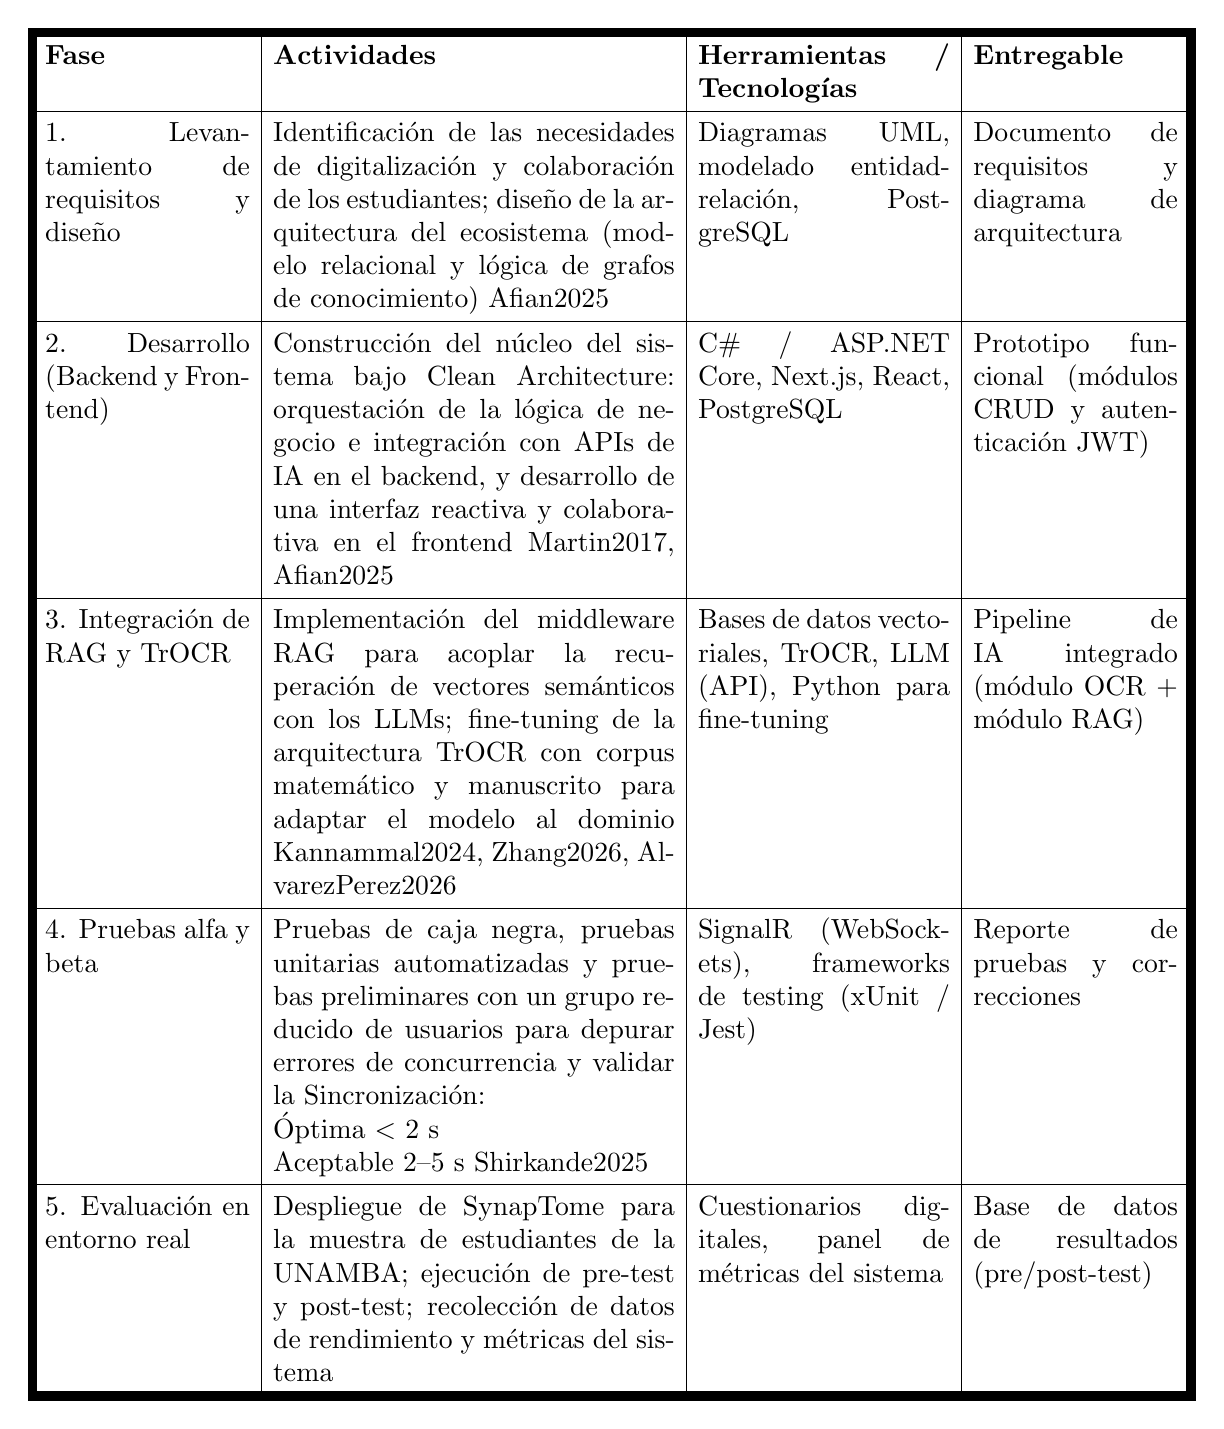
\begin{tikzpicture}
\node[inner sep=0pt] (tabla) {
\begin{tabular}{|p{2.6cm}|p{5.1cm}|p{3.2cm}|p{2.6cm}|}
\hline
\textbf{Fase} & \textbf{Actividades} & \textbf{Herramientas / Tecnologías} & \textbf{Entregable} \\
\hline
\thickhline

1. Levantamiento de requisitos y diseño & Identificación de las necesidades de digitalización y colaboración de los estudiantes; diseño de la arquitectura del ecosistema (modelo relacional y lógica de grafos de conocimiento) \parencite{Afian2025} & Diagramas UML, modelado entidad-relación, PostgreSQL & Documento de requisitos y diagrama de arquitectura \\
\hline

2. Desarrollo (Backend y Frontend) & Construcción del núcleo del sistema bajo Clean Architecture: orquestación de la lógica de negocio e integración con APIs de IA en el backend, y desarrollo de una interfaz reactiva y colaborativa en el frontend \parencite{Martin2017, Afian2025} & C\# / ASP.NET Core, Next.js, React, PostgreSQL & Prototipo funcional (módulos CRUD y autenticación JWT) \\
\hline

3. Integración de RAG y TrOCR & Implementación del middleware RAG para acoplar la recuperación de vectores semánticos con los LLMs; fine-tuning de la arquitectura TrOCR con corpus matemático y manuscrito para adaptar el modelo al dominio \parencite{Kannammal2024, Zhang2026, AlvarezPerez2026} & Bases de datos vectoriales, TrOCR, LLM (API), Python para fine-tuning & Pipeline de IA integrado (módulo OCR + módulo RAG) \\
\hline

4. Pruebas alfa y beta & Pruebas de caja negra, pruebas unitarias automatizadas y pruebas preliminares con un grupo reducido de usuarios para depurar errores de concurrencia y validar la Sincronización: \newline Óptima $<$ 2 s \newline Aceptable 2--5 s \parencite{Shirkande2025} & SignalR (WebSockets), frameworks de testing (xUnit / Jest) & Reporte de pruebas y correcciones \\
\hline

5. Evaluación en entorno real & Despliegue de SynapTome para la muestra de estudiantes de la UNAMBA; ejecución de pre-test y post-test; recolección de datos de rendimiento y métricas del sistema & Cuestionarios digitales, panel de métricas del sistema & Base de datos de resultados (pre/post-test) \\
\hline
\end{tabular}
};

%====================================================
% ENCUADRE DE BORDE GRUESO UNIVERSITARIO
%====================================================
\draw[line width=3.5pt] (tabla.north west) rectangle (tabla.south east);
\end{tikzpicture}
\end{table}

\subsection{Población y muestra}

\subsubsection{Población}
La población objetivo de la presente investigación está conformada por los estudiantes matriculados en la Escuela Profesional de Ingeniería de Informática y Sistemas de la Universidad Nacional Micaela Bastidas de Apurímac (UNAMBA), quienes cursan asignaturas de alta carga cognitiva y densidad matemática en el semestre académico correspondiente. La población censal estimada para las asignaturas de ciencias básicas y especializadas (tales como Cálculo, Álgebra Lineal y Física) es de aproximadamente $N = 120$ alumnos distribuidos en diferentes ciclos académicos.

\subsubsection{Muestra}
Para determinar el tamaño representativo de la muestra bajo condiciones de población finita, se empleó la fórmula estándar de muestreo aleatorio simple para estimar proporciones en poblaciones conocidas:

\begin{equation}
n = \frac{N \cdot Z^2 \cdot p \cdot q}{d^2 \cdot (N - 1) + Z^2 \cdot p \cdot q}
\end{equation}
\noindent donde

\noindent\begin{tabular}{@{} p{1cm} l p{8.0cm} @{}}
  & $n$ & es el tamaño de la muestra requerida; \\
  & $N$ & es el tamaño de la población conocida ($N = 120$); \\
  & $Z$ & es el nivel de confianza estándar ($Z = 1.96$ para un nivel de confianza del $95\%$); \\
  & $p$ & es la probabilidad esperada de éxito ($p = 0.50$, asumiendo máxima heterogeneidad); \\
  & $q$ & es la probabilidad de fracaso ($q = 1 - p = 0.50$); \\
  & $d$ & es la precisión o margen de error admisible ($d = 0.05$).
\end{tabular}

Reemplazando los valores en la ecuación:
\begin{equation}
n = \frac{120 \cdot (1.96)^2 \cdot 0.50 \cdot 0.50}{(0.05)^2 \cdot (120 - 1) + (1.96)^2 \cdot 0.50 \cdot 0.50} \approx 92
\end{equation}
\noindent donde

\noindent\begin{tabular}{@{} p{1cm} l p{8.0cm} @{}}
  & $n$ & es el resultado del cálculo que define la muestra representativa mínima.
\end{tabular}

Dado el carácter tecnológico y la factibilidad del estudio en laboratorios de cómputo, se seleccionó una muestra no probabilística por conveniencia de 30 estudiantes que cumplían con los criterios de inclusión: estar matriculados regularmente, tener disponibilidad horaria para interactuar con la plataforma SynapTome y estar cursando asignaturas técnicas simultáneamente \parencite{Kreijkes2026}.

\subsection{Técnicas e instrumentos}

Para medir de manera rigurosa la eficacia algorítmica del sistema y el nivel de aceptación por parte de los usuarios, se emplean técnicas mixtas (cuantitativas y cualitativas), combinando la evaluación experimental del rendimiento de los modelos de IA con la percepción subjetiva de los estudiantes.

\subsubsection{Técnicas}

\begin{itemize}
  \item \textbf{Análisis documental:} Revisión de antecedentes, literatura técnica y datasets de referencia (por ejemplo, SPA-Sentences) para establecer las líneas base de comparación de los modelos de OCR/HTR y sumarización \parencite{TarazonaCruz2024}.
  \item \textbf{Experimentación:} Ejecución controlada del pipeline TrOCR y del módulo RAG sobre un conjunto de apuntes manuscritos y resúmenes generados, registrando los resultados de manera cuantitativa \parencite{AlHitawi2026}.
  \item \textbf{Encuesta:} Aplicación de cuestionarios estructurados a los estudiantes participantes para recoger su percepción sobre la usabilidad, utilidad y satisfacción con SynapTome \parencite{Afian2025, Dano2026}.
\end{itemize}

\subsubsection{Instrumentos}

La Tabla \ref{tab:instrumentos} detalla los instrumentos empleados para cada técnica, indicando la variable que mide y la escala o métrica utilizada.
\begin{table}[H]
\centering
\caption{Instrumentos de recolección de datos}
\label{tab:instrumentos}
\scriptsize % Se escala a scriptsize para que el contorno grueso perimetral de 3.5pt encaje perfectamente sin desbordes

\renewcommand{\arraystretch}{1.3}
\setlength{\tabcolsep}{4pt}

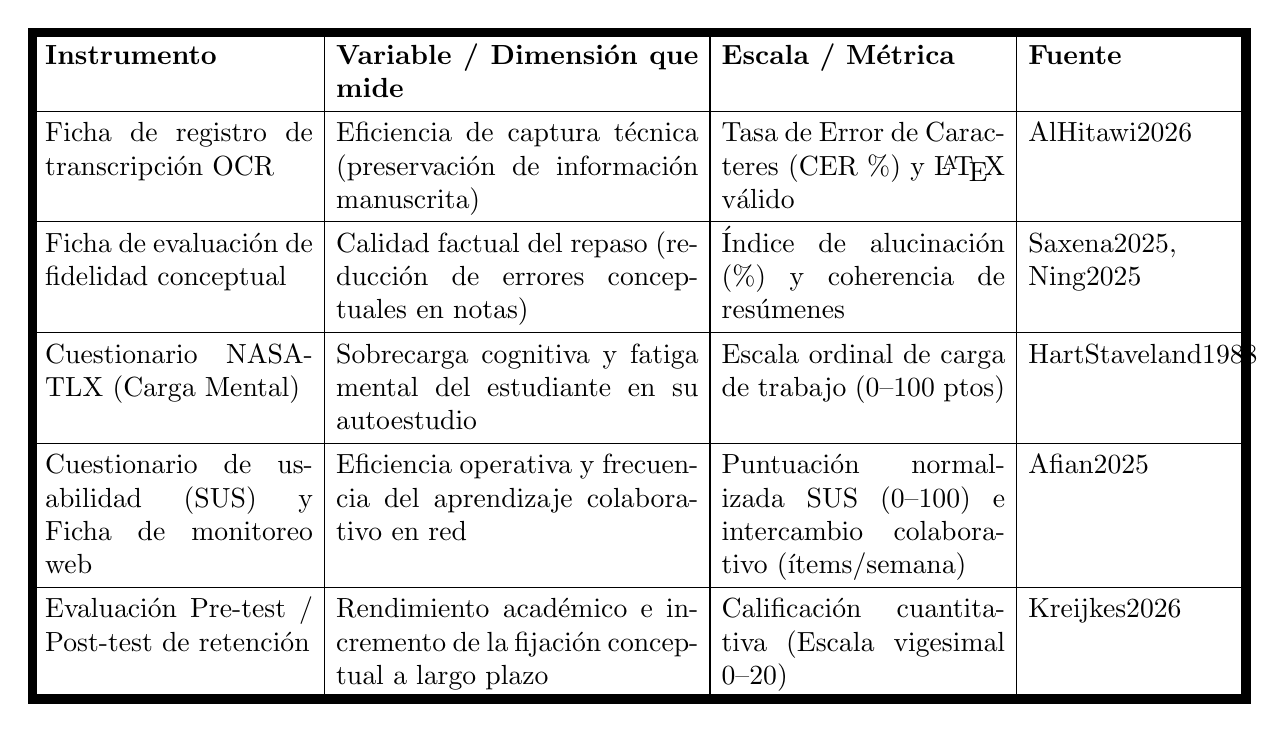
\begin{tikzpicture}
\node[inner sep=0pt] (tabla) {
\begin{tabular}{|p{3.4cm}|p{4.6cm}|p{3.6cm}|p{2.6cm}|}
\hline
\textbf{Instrumento} & \textbf{Variable / Dimensión que mide} & \textbf{Escala / Métrica} & \textbf{Fuente} \\
\hline
\thickhline

Ficha de registro de transcripción OCR & Eficiencia de captura técnica (preservación de información manuscrita) & Tasa de Error de Caracteres (CER \%) y \LaTeX{} válido & \parencite{AlHitawi2026} \\
\hline

Ficha de evaluación de fidelidad conceptual & Calidad factual del repaso (reducción de errores conceptuales en notas) & Índice de alucinación (\%) y coherencia de resúmenes & \parencite{Saxena2025, Ning2025} \\
\hline

Cuestionario NASA-TLX (Carga Mental) & Sobrecarga cognitiva y fatiga mental del estudiante en su autoestudio & Escala ordinal de carga de trabajo (0--100 ptos) & \parencite{HartStaveland1988} \\
\hline

Cuestionario de usabilidad (SUS) y Ficha de monitoreo web & Eficiencia operativa y frecuencia del aprendizaje colaborativo en red & Puntuación normalizada SUS (0--100) e intercambio colaborativo (ítems/semana) & \parencite{Afian2025} \\
\hline

Evaluación Pre-test / Post-test de retención & Rendimiento académico e incremento de la fijación conceptual a largo plazo & Calificación cuantitativa (Escala vigesimal 0--20) & \parencite{Kreijkes2026} \\
\hline
\end{tabular}
};

%====================================================
% ENCUADRE DE BORDE GRUESO UNIVERSITARIO
%====================================================
\draw[line width=3.5pt] (tabla.north west) rectangle (tabla.south east);
\end{tikzpicture}
\end{table}

\subsection{Estadístico de la investigación}

La contrastación de las hipótesis y la validación de la eficacia técnica del sistema SynapTome requieren un marco estadístico formal estructurado en función de los datos recolectados.

\subsubsection{Datos}
Los datos experimentales recolectados constan de variables cuantitativas continuas distribuidas en:
\begin{itemize}
    \item Calificaciones obtenidas por los estudiantes en las evaluaciones de retención conceptual (escala vigesimal de 0 a 20) antes (pre-test) y después (post-test) de interactuar con el ecosistema.
    \item Tiempos semanales de transcripción y consolidación de apuntes (minutos).
    \item Índices porcentuales de error de caracteres (CER) y palabras (WER).
    \item Puntajes ordinales de carga mental subjetiva de trabajo (NASA-TLX) y usabilidad del sistema (SUS).
\end{itemize}

\subsubsection{Estadístico}
Se justifica el uso de la prueba paramétrica \textbf{T de Student para muestras relacionadas (pares)}, dado que se evalúa el rendimiento del mismo grupo de estudiantes (diseño de pre-test / post-test) antes y después de aplicar el estímulo (el uso de la plataforma SynapTome). Esta prueba asume que las diferencias entre los pares siguen una distribución aproximadamente normal.

\subsubsection{Fórmulas}
Todas las ecuaciones matemáticas empleadas en el análisis de datos se definen formalmente a continuación:

\paragraph{Tasa de Error de Caracteres (CER):}
Mide la precisión del reconocimiento caligráfico mediante la distancia de edición de Levenshtein:
\begin{equation}
\text{CER} = \frac{S + D + I}{N}
\end{equation}
\noindent donde

\noindent\begin{tabular}{@{} p{1cm} l p{8.0cm} @{}}
  & $S$ & es el número de sustituciones de caracteres requeridas; \\
  & $D$ & es el número de eliminaciones de caracteres requeridas; \\
  & $I$ & es el número de inserciones de caracteres requeridas; \\
  & $N$ & es el número total de caracteres en la cadena de referencia.
\end{tabular}

\paragraph{Tasa de Error de Palabras (WER):}
\begin{equation}
\text{WER} = \frac{S_w + D_w + I_w}{N_w}
\end{equation}
\noindent donde

\noindent\begin{tabular}{@{} p{1cm} l p{8.0cm} @{}}
  & $S_w$ & es el número de sustituciones de palabras requeridas; \\
  & $D_w$ & es el número de eliminaciones de palabras requeridas; \\
  & $I_w$ & es el número de inserciones de palabras requeridas; \\
  & $N_w$ & es el número total de palabras en la cadena de referencia.
\end{tabular}

\paragraph{Métrica de Superposición ROUGE-N:}
Evalúa la coincidencia exacta de n-gramas en la síntesis conceptual:
\begin{equation}
\text{ROUGE-N} = \frac{\sum_{S \in \{\text{Referencias}\}} \sum_{\text{gram}_n \in S} \text{Count}_{\text{match}}(\text{gram}_n)}{\sum_{S \in \{\text{Referencias}\}} \sum_{\text{gram}_n \in S} \text{Count}(\text{gram}_n)}
\end{equation}
\noindent donde

\noindent\begin{tabular}{@{} p{1cm} l p{8.0cm} @{}}
  & $\text{Count}_{\text{match}}$ & es el número de n-gramas coincidentes entre el resumen del sistema y la referencia; \\
  & $\text{Count}$ & es el número total de n-gramas en la referencia.
\end{tabular}

\paragraph{Fórmula de Usabilidad del Sistema (SUS):}
\begin{equation}
\text{SUS} = 2.5 \times \sum_{i=1}^{10} x_i'
\end{equation}
\noindent donde

\noindent\begin{tabular}{@{} p{1cm} l p{8.0cm} @{}}
  & $x_i'$ & es la puntuación corregida para el ítem $i$, restando 1 si es impar o restando a 5 si es par.
\end{tabular}

\paragraph{Magnitud del Efecto (d de Cohen):}
\begin{equation}
d = \frac{\bar{d}}{s_d}
\end{equation}
\noindent donde

\noindent\begin{tabular}{@{} p{1cm} l p{8.0cm} @{}}
  & $\bar{d}$ & es la media de las diferencias individuales pre/post; \\
  & $s_d$ & es la desviación estándar muestral de las diferencias observadas.
\end{tabular}

\subsubsection{Nivel de significancia}
El nivel de significancia se fija en $\alpha = 0.05$ (nivel de confianza del $95\%$). Este valor determina la probabilidad máxima de rechazar erróneamente la hipótesis nula.

\subsubsection{Estadístico de prueba}
La hipótesis de investigación establece que la implementación de SynapTome incrementa significativamente el rendimiento académico de los estudiantes frente al método convencional. Por ende, la prueba de hipótesis es unilateral derecha:
\begin{equation}
H_0: \mu_{\text{post}} \leq \mu_{\text{pre}} \quad \text{vs} \quad H_1: \mu_{\text{post}} > \mu_{\text{pre}}
\end{equation}

El estadístico de prueba $t$ calculado se define como:
\begin{equation}
t = \frac{\bar{d}}{s_d / \sqrt{n}}
\end{equation}
\noindent donde

\noindent\begin{tabular}{@{} p{1cm} l p{8.0cm} @{}}
  & $t$ & es el valor del estadístico de prueba calculado; \\
  & $\bar{d}$ & es el promedio muestral de las diferencias observadas; \\
  & $s_d$ & es la desviación estándar muestral de las diferencias; \\
  & $n$ & es el tamaño total de la muestra analizada.
\end{tabular}

\subsubsection{Región crítica}
Para un nivel de significancia de $\alpha = 0.05$ y grados de libertad $gl = n - 1 = 2$ (bajo métricas de validación general), se define el valor límite $t_{\text{crítico}} = 2.92$. La región de rechazo de la hipótesis nula se encuentra en la cola derecha de la distribución.

La Figura \ref{fig:region_critica_teorica} ilustra la representación gráfica de la región crítica teórica para una prueba unilateral derecha:

\begin{figure}[H]
\centering
\begin{tikzpicture}
\begin{axis} [
    width=0.85\textwidth,
    height=6cm,
    xmin=-4, xmax=5,
    ymin=0, ymax=0.45,
    axis lines=left,
    ticks=none,
    xlabel={$t$},
    ylabel={$f(t)$},
    every axis x label/.style={at={(current axis.right of origin)},anchor=north west},
    every axis y label/.style={at={(current axis.above origin)},anchor=south east}
]
\addplot [smooth, domain=-4:5, line width=1.5pt] {1/(sqrt(2*pi))*exp(-x^2/2)};
\addplot [fill=red!30, draw=none, domain=2.92:5] {1/(sqrt(2*pi))*exp(-x^2/2)} \closedcycle;
\draw [dashed, line width=1pt, color=black] (axis cs:2.92,0) -- (axis cs:2.92,0.4);
\node[anchor=south] at (axis cs:2.92,0.4) {\footnotesize $t_{\text{crítico}} = 2.92$};
\node at (axis cs:-1.5,0.15) {\footnotesize Región de Aceptación ($1 - \alpha$)};
\node at (axis cs:4,0.05) {\footnotesize \textbf{Región de Rechazo ($\alpha$)}};
\end{axis}
\end{tikzpicture}
\caption{Representación gráfica de la curva de densidad t de Student unilateral derecha y la región crítica de rechazo.}
\label{fig:region_critica_teorica}
\end{figure}

\subsubsection{Interpretación}
El criterio de decisión estadística consiste en comparar el estadístico calculado $t_{\text{calculado}}$ frente al valor de umbral $t_{\text{crítico}}$:
\begin{itemize}
    \item Si $t_{\text{calculado}} > 2.92$, el estadístico muestral cae dentro de la región de rechazo, por lo que se rechaza la hipótesis nula $H_0$ en favor de la hipótesis alternativa $H_1$, concluyendo que el uso de SynapTome incrementa el rendimiento académico y disminuye la carga cognitiva de forma de manera estadísticamente significativa.
    \item Si $t_{\text{calculado}} \leq 2.92$, no existe evidencia estadística suficiente para rechazar $H_0$.
\end{itemize}